\documentclass[]{article}
\usepackage[pdftex,paperwidth=434pt,paperheight=244pt,noheadfoot,left=0pt,top=0pt]{geometry}
\usepackage{graphicx}

\begin{document}
\noindent
%\scalebox{0.8819}[0.8966]{
\begin{picture}(432,243)
\put(-108,-482){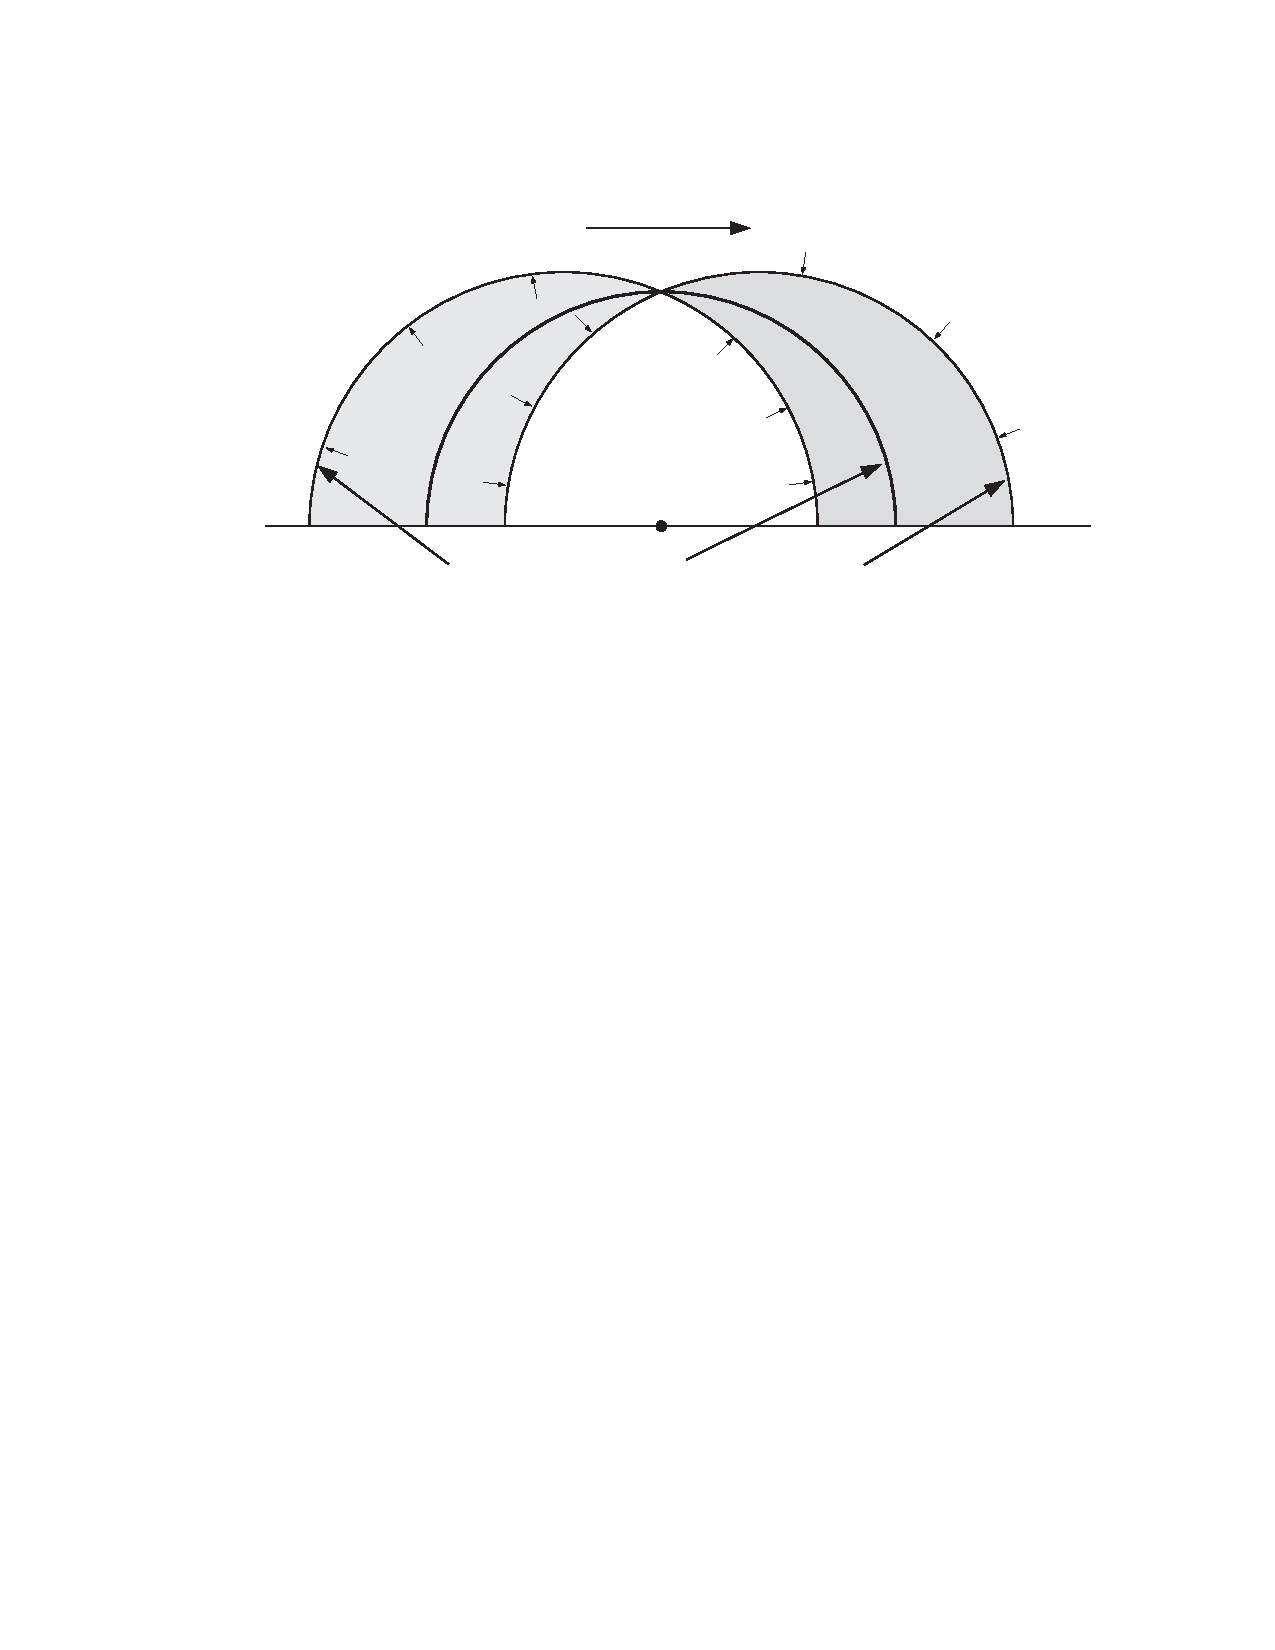
\includegraphics[width=8.5in]{PDFnotext/Figure13_4.pdf}}
\put(209,209){\boldmath{P}}
\put(387,64){$\theta=0$}
\put(15,64){$\theta=\pi$}
\put(200,64){$r=0$}
\put(62,31){Top Sheet}
\put(62,21){Apparent Horizon}
\put(290,31){Bottom Sheet}
\put(290,21){Apparent Horizon}
\put(175,31){Minimal Surface}
\put(175,21){$r=a$}
\end{picture}
%}
\end{document}
